% Source: source/普通高考/2007/2007湖南理.pdf, page 2, question 19.
% Spatial coordinates from the given OA, AB, PH and sin(theta); D,E are schematic road points.
% Solid segments: OA, OE, AB, DP, BP. Dashed segment: PH (vertical drop to the horizontal plane).
% Labels: O left, A above, E/D/B below, P right, H below; no photographic terrain texture.
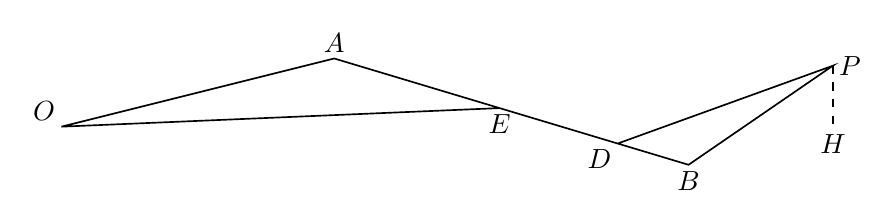
\begin{tikzpicture}[x={(3cm,-.9cm)},y={(-2cm,-.5cm)},z={(0cm,2cm)},line width=.6pt,font=\normalsize]
\coordinate (A) at (0,0,0);
\coordinate (B) at (1.5,0,0);
\coordinate (O) at (0,{sqrt(3)},0);
\coordinate (P) at (1.5,{-sqrt(21)/5},.4);
\coordinate (H) at (1.5,{-sqrt(21)/5},0);
\coordinate (D) at (1.2,0,0);
\coordinate (E) at (.7,0,0);
\draw (O)--(A)--(B)--(P)--(D) (O)--(E);
\draw[dashed] (P)--(H);
\node[above left,inner sep=2pt] at (O) {$O$};
\node[above,inner sep=2pt] at (A) {$A$};
\node[below,inner sep=2pt] at (E) {$E$};
\node[below left,inner sep=2pt] at (D) {$D$};
\node[below,inner sep=2pt] at (B) {$B$};
\node[right,inner sep=2pt] at (P) {$P$};
\node[below,inner sep=2pt] at (H) {$H$};
\end{tikzpicture}
